%%%%%%%%%%%%%%%%%%%%%%%%%%%%%%%%%%%%%%%%%
% Structured General Purpose Assignment
% LaTeX Template
%
% This template has been downloaded from:
% http://www.latextemplates.com
%
% Original author:
% Ted Pavlic (http://www.tedpavlic.com)
%
% Note:
% The \lipsum[#] commands throughout this template generate dummy text
% to fill the template out. These commands should all be removed when 
% writing assignment content.
%
%%%%%%%%%%%%%%%%%%%%%%%%%%%%%%%%%%%%%%%%%

\documentclass{article}

\usepackage{fancyhdr} % Required for custom headers
\usepackage{lastpage} % Required to determine the last page for the footer
\usepackage{extramarks} % Required for headers and footers
\usepackage{graphicx} % Required to insert images
\usepackage[utf8]{inputenc}

% Margins
\topmargin=-0.45in
\evensidemargin=0in
\oddsidemargin=0in
\textwidth=6.5in
\textheight=9.0in
\headsep=0.25in 

\linespread{1.1} % Line spacing



\setlength\parindent{0pt} % Removes all indentation from paragraphs

%----------------------------------------------------------------------------------------
%	DOCUMENT STRUCTURE COMMANDS
%	Skip this unless you know what you're doing
%----------------------------------------------------------------------------------------

% Header and footer for when a page split occurs within a problem environment
\newcommand{\enterProblemHeader}[1]{
\nobreak\extramarks{#1}{#1 continued on next page\ldots}\nobreak
\nobreak\extramarks{#1 (continued)}{#1 continued on next page\ldots}\nobreak
}

% Header and footer for when a page split occurs between problem environments
\newcommand{\exitProblemHeader}[1]{
\nobreak\extramarks{#1 (continued)}{#1 continued on next page\ldots}\nobreak
\nobreak\extramarks{#1}{}\nobreak
}

\setcounter{secnumdepth}{0} % Removes default section numbers
\newcounter{homeworkProblemCounter} % Creates a counter to keep track of the number of problems

%----------------------------------------------------------------------------------------
%	NAME AND CLASS SECTION
%----------------------------------------------------------------------------------------

\newcommand{\lessonNumber}[1]{Lezione\ \##1} % Assignment title
\newcommand{\lessonDate}[4]{#1,\ #2\ #3\ #4} % Due date
\newcommand{\lessonCourse}[1]{#1} % Course/class
\newcommand{\lessonTime}[1]{#1} % Class/lecture time
\newcommand{\lessonTeacher}[1]{#1} % Teacher/lecturer
\newcommand{\lessonAuthor}[1]{#1} % Your name

\begin{document}

\section{Diagrammi delle classi(3)}

Una classe è una descrizione di qualcosa e l'oggetto è un'istanza che rispetta questa descrizione. Si passa dalla descrizione a qualcosa di tangibile. I diagrammi delle classi modellano un concetto ed sono indipendenti dal linguaggio di programmazione con cui andrò a implementare. La prima cosa che andremo a definire di una classe sono i suoi attributi, che vanno scritti nella parte centrale.

\begin{center}

\texttt{Visibilità nome : tipo [molteplicità] = default [proprietà aggiuntive]}

\end{center}

Questa è la segnatura per la visibilità degli attributi:

\begin{itemize}

	\item \textbf{+}, pubblica;
	\item \textbf{-}, privata;
	\item \textbf{\#}, protetta.

\end{itemize}

L'attributo può essere anche espresso come \textbf{associazione} tra due tipi. Questo si fa con una freccia orientata dalla classe che contiene una copia dell'altro tipo è bene cercare di metterli privati.\\
Associazioni senza verso sono bidirezionali, evitarle se possibile e usare un nome non un verbo che le descrivano. Si utilizzano gli attributi testuali per i tipi primitivi, mentre si utilizzano le associazioni quando ci si riferisce a due classi del nostro dominio.\\
Se abbiamo molteplicità superiore a 1 significa che abbiamo una collezione (array, liste, ...). Le proprietà sono gli attributi e le associazioni, le operazioni sono ciò che la classe espone verso l'esterno, sono i "servizi" della classe.

\begin{center}

\texttt{Visibilità nome (lista-parametri} : tipo-ritorno {proprietà aggiuntive\}}\\
\texttt{Lista-proprietà := direzione nome : tipo = default}

\end{center}


Le \textbf{query} sono tutte le operazioni che non modificano l'oggetto di invocazione, a differenza dei metodi modificatori. Operazione != metodo, concetto differente in presenza di polimorfismo.\\

\textbf{Commenti e note}

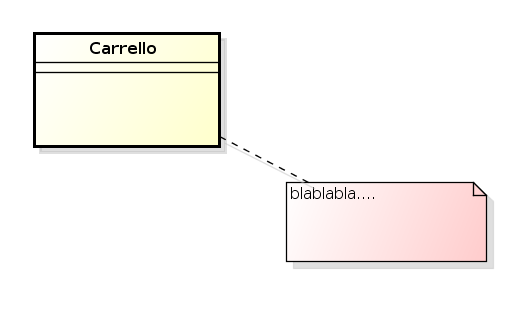
\includegraphics[width=0.5\columnwidth]{img9} % Example image
\\
Un concetto fondamentale è la dipendenza fra due tipi. Una classe A dipende da B se una modifica fatta a B implica una modifica ad A. Le dipendenze vanno minimizzate, perchè le classi devono essere autoconsistenti. Più dipendenze ho e più una modifica può creare \textit{side-effect} su un'altra classe (problemi in fase di manutenzione). Un modo per minimizzare le dipendenze è l'uso di interfacce.\\
Le dipendenze in UML sono di vario tipo, c'è bisogno di un classificatore, al fine di comprenderla meglio. Questo si inserisce come etichetta nella freccia.\\

\pagebreak

\textbf{Relazioni:}
\begin{itemize}
	\item \textit{L'aggregazione} si identifica con la frase "\textit{parte di...}", gli aggregati possono essere condivisi. Viene rappresentato con un diamante vuoto.
	\item \textit{La composizione} è come l'aggregazione ma le istanze i un'aggregazione possono appartenere solo ad un aggregato. Solo l'oggetto intero può creare e distruggere le sue parti.
\end{itemize}


\begin{center}

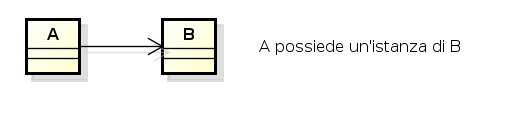
\includegraphics[width=0.5\columnwidth]{img11} % Example image

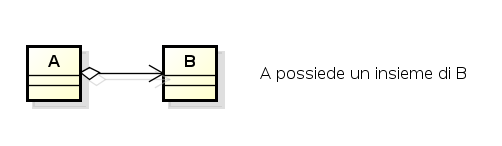
\includegraphics[width=0.5\columnwidth]{img12} % Example image

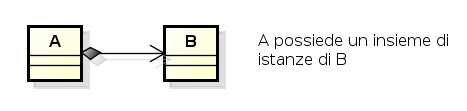
\includegraphics[width=0.5\columnwidth]{img13} % Example image

\end{center}

Si possono aggiungere ulteriori attributi alle associazioni

La generalizzazione è un concetto molto importante perchè descrive l'ereditarietà, uno dei concetti fondamentali della programmazione a oggetti. A generalizza B se ogni oggetto di B è anche un oggetto di A. Sottotipo != Sottoclasse. L'ereditarietà multipla è supportata, attenzione da usare pochissimo.

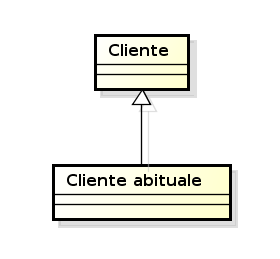
\includegraphics[width=0.3\columnwidth]{img15} 
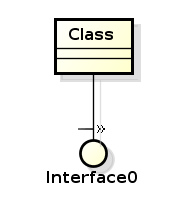
\includegraphics[width=0.3\columnwidth]{img16} % Example image% Example image

Per le classi astratte e altro si usa il \textit{corsivo}, la classe non può essere instanziata perché ha delle operazioni che non possiedono l'implementazione, anche se ne può possedere alcune implementate.\\

Un altro concetto è quello di \textbf{interfaccia}, che non è una classe (al massimo è un tipo) ed è priva di implementazione. Il loro scopo è definire un contratto che le classi che la implementeranno devono assolutamente fornire.

Caratteristiche varie sui diagrammi delle classi:
\begin{itemize}
	\item \textbf{Attributi o operazioni statiche:} non associati ad un oggetto ma al tipo, vanno sottolineati. L'utilizzo di variabili e metodi statici va normalmente evitato, perchè si rischia di tornare alla programmazione procedurale;
	\item \textbf{Proprietà read-only:}, non deve fornire i servizi di scrittura su quella classe;
	\item \textbf{Proprietà frozen:} significa che è una costante, l'attributo non può essere modificato;
	\item \textbf{Classi parametriche:} come un template in C++, si rappresentano con un rettangolo con bordo tratteggiato in alto a destra della classe. 
	\item \textbf{Classi attive:} sono classi che possono essere eseguite (in Java le classi che estendono \textit{Thread}).
 
\end{itemize}

\end{document}